\documentclass[11pt,a4paper]{article}
\usepackage{graphicx}
\usepackage{listings}
\usepackage{hyperref}
\hypersetup{
    colorlinks,
    citecolor=black,
    filecolor=black,
    linkcolor=black,
    urlcolor=black
}
\usepackage{xcolor}
\lstset{basicstyle=\ttfamily,
  showstringspaces=false,
  commentstyle=\color{red},
  keywordstyle=\color{blue}
}
\usepackage{float}
\title{Comparison of symmetric ciphers in OpenSSL \\ HW1 - CNS Sapienza}

\author{Edoardo Puglisi 1649359} 
\date{04/11/2019}

\begin{document}
\lstset{breaklines=true}
	
\maketitle
\tableofcontents
\clearpage

\section{Overview}
The following experiment consists of comparing encryption/decryption speeds of multiple symmetric ciphers with different operating modes.It has the purpose to find correlations between file size and efficiency of different ciphers. 

\section{Ciphers}
Here the list of chipers used for the experiment with brief descriptions.
\begin{itemize}
    \item \textbf{DES:} uses a 56-bits key and for this is highly insecure, but it was highly influential for modern cryptography. DES takes a fized-length plaintext and transforms it into a ciphertex of same size using a serie of complicated operations also with the usage of key to costumize the transformations and make them more secure.
  \item \textbf{AES:} standing for Advanced Encryption Standard, AES is an algorithm which became standard for the U.S. National Institute of Standards and Technology (NIST).
  Plaintext is represented as a block matrix A.
  Steps: 
  \begin{enumerate}
      \item Key expansion - the cipher key is divided in multiple round key. One round-key block per round + 1
      \item First step - AddRoundKey = bitwise XOR with byte of state and round-key block
      \item Rounds - \begin{itemize}
          \item Substitution = $A[i,j]$ is swapped with $A[i,j]^{-1}$
          \item RowShift = row i is shifted of i-1 positions.
          \item Multiplication =  multiply every column with an invertible polynomial $03x^{3}+01x^{2}+01x+02(mod(x^{4}+1))$
          \item AddRoundKey
      \end{itemize}
      \item Final round - same steps as before but without Multiplication
  \end{enumerate}
  \item \textbf{Camellia:} algorithm developed by Mitsubishi Electric and NNT of Japan. It is comparable to AES in term of security and processing abilities. It was designed to be suitable for both software and hardware implementations. Composed by 18/24 rounds, every six rounds it apply a FL function (or its inverse) i.e. a logical transformation layer.
  \item \textbf{Aria:} developed by a group of researchers of South Korea, is based on AES interface. This algorithm uses a substitution-permutation network derived from AES.
  
\end{itemize}

\clearpage

\section{Operating modes}
Short description of operating modes used by all ciphers.
\begin{itemize}
    \item \textbf{ECB:} Electronic Code Block, the simplest operating mode. Plaintext managed 64bit at time, each block encrypted with same key. If needed padding bits are added to reach block size. Process can be parallelized and there isn't errors propagation. Data integrity not guaranteed due to the fact that attackers can swap blocks positions and insecure against bruteforce attacks.
    \begin{figure}[H]
        \centering
            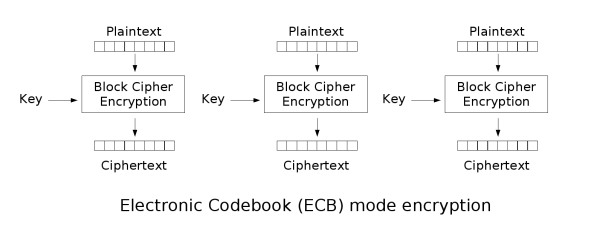
\includegraphics[width=\textwidth]{ecb-hw1-1649359.png}
    \end{figure}
    \item \textbf{CBC:} the basic idea is that a plaintext block if repeated will produce different cipher blocks. To each plaintext block is applied the XOR operand with the previous ciphertext block.
    \begin{figure}[H]
        \centering
            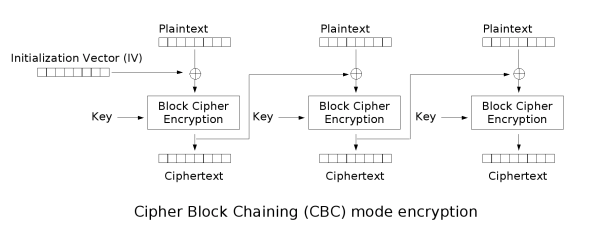
\includegraphics[width=\textwidth]{cbc-hw1-1649359.png}
    \end{figure}
\end{itemize}

\clearpage

\section{Code}
Code description.
\lstinputlisting[language=bash]{script-hw1-1649359.sh}
The script used for the experiment consists of 10 iterations of encryption and 10 iterations of decryption for every cipher on files of different sizes. In addition for every cipher two different operating mode have been used (ECB and CBC).
Encryption and decryption times are written on a csv file used to draw the graphs.

\clearpage
\section{Results}
Here the resulting graphs.

\begin{figure}[H]
    \centering
        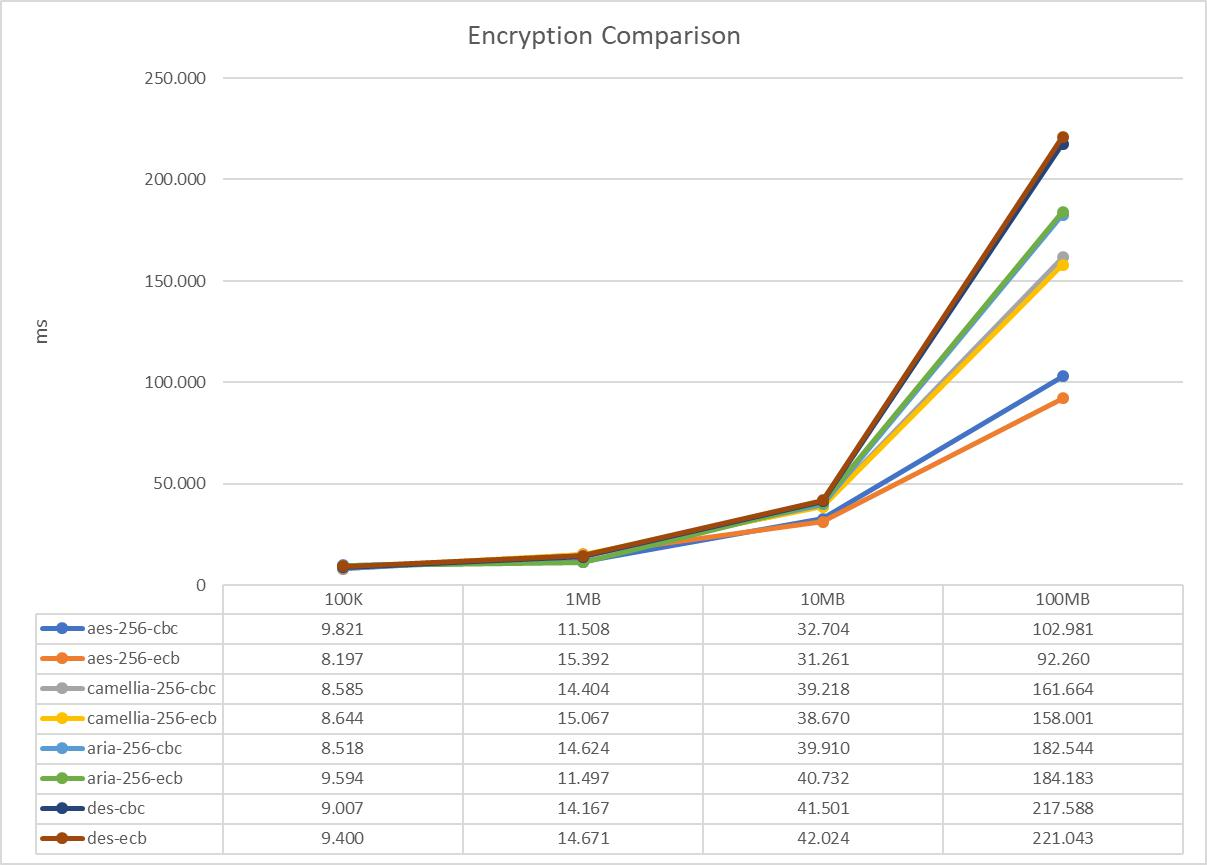
\includegraphics[width=\textwidth]{enc-hw1-1649359.jpg}
\end{figure}
\begin{figure}[h]
    \centering
        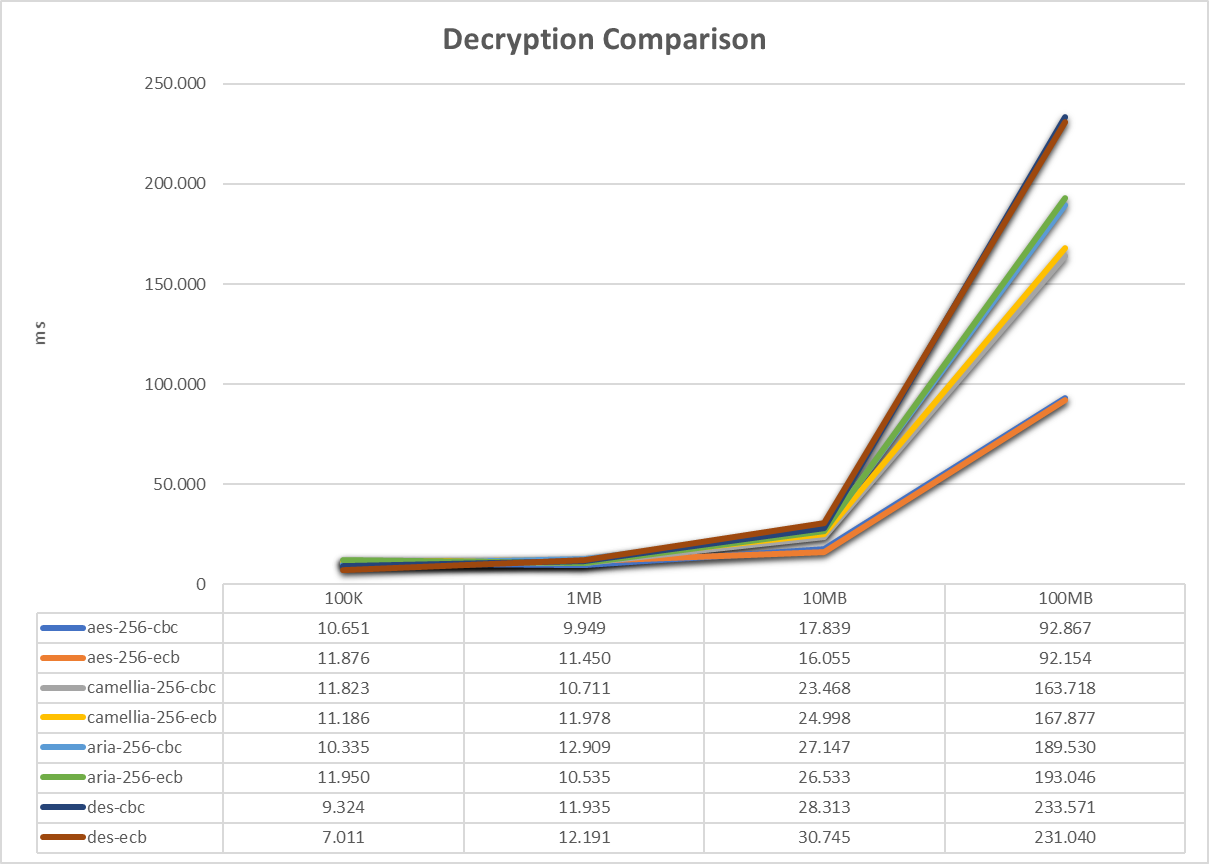
\includegraphics[width=\textwidth]{dec-hw1-1649359.jpg}
\end{figure}

We can see that AES algorithm is the best in terms of efficiency in both encryption and decryption. The difference between operating modes doesn't influence much computing time and this means that CBC, besides being safer than ECB, doesn't effect encryption and decryption efficiency.
Above 10MB, file size starts effecting the computation, showing an huge increment of computing time in all ciphers.

\begin{figure}[h]
    \centering
        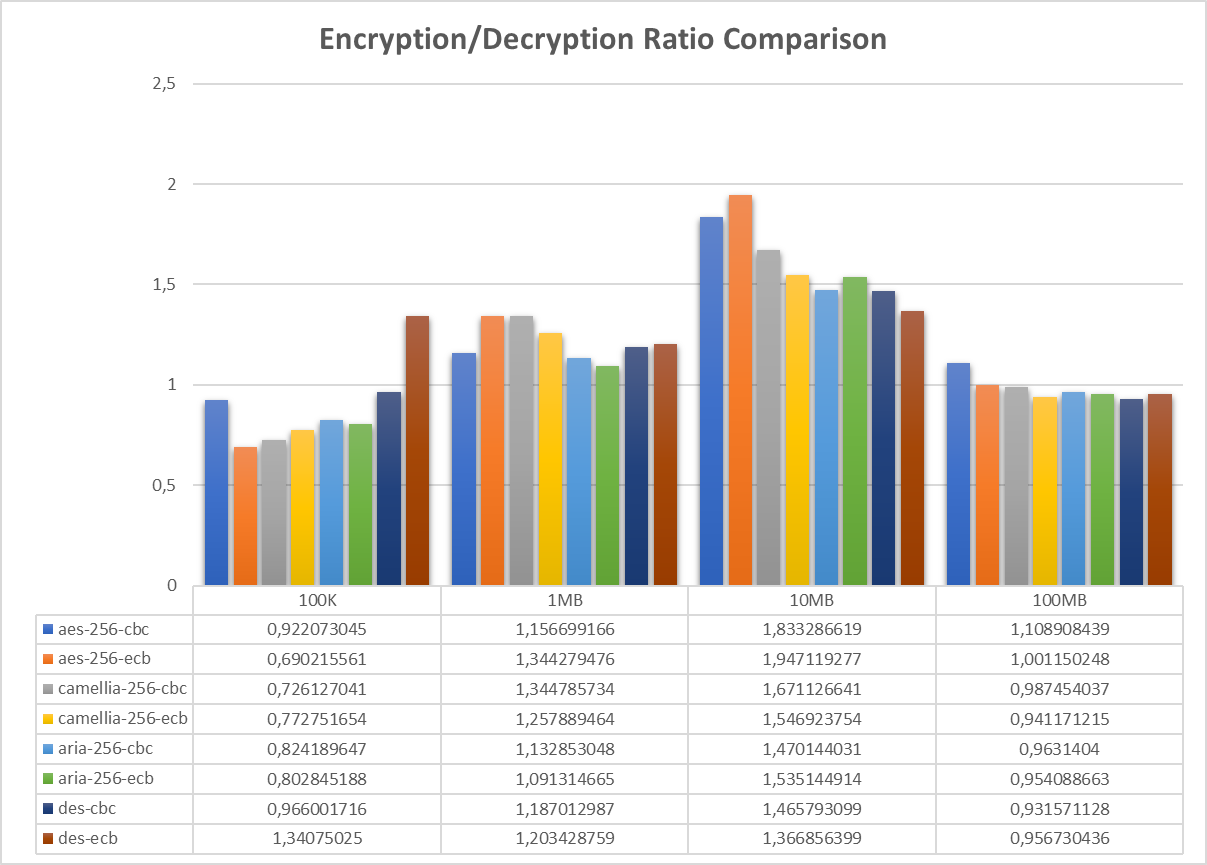
\includegraphics[width=\textwidth]{ratio-hw1-1649359.jpg}
\end{figure}

About the encryption/decryption ratio we can see that the main differences can be found on small size file where operating mode influences a lot the ratio: for example AES CBC has a ratio much higher than AES EBC on 100K files.
We have an huge increment of ratio in all ciphers and operating modes for 10MB files that decreases again on 100MB files where becomes almost equal for all ciphers.

\end{document}
